\subsection{Road Generation}
The fundamental infrastructure of a city is the road network and as such, it was important to get this right early on in development, and the generator had to be both flexible and also offer realistic-looking results.
To generate the road network for the city, a RoadGenerator function was implemented which takes the terrain and the population map as inputs.
These parameters are then used to produce a road network as output, as is shown in Table~\ref{table:def_roadgen}.

\begin{table}[H]
  \centering
  \begin{tabular}{lllll}
    \textbf{Input} & & \textbf{Function} & & \textbf{Output} \\
    \midrule
    \textit{Terrain, PopulationMap, Markers} & $\rightarrow$ & \textbf{RoadGenerator} & $\rightarrow$ & \textit{RoadNetwork} \\
    \bottomrule
  \end{tabular}

  \caption{Definition of the RoadGenerator which is responsible for generating road networks.}
  \label{table:def_roadgen}
\end{table}
\vspace{-0.4cm}

Two major approaches were considered when designing the road generator.
The first were based on a recursive approach where the world were divided into multiple cells with roads placed between the cells.
However, this type of algorithm did not provide realistic-looking results and, while being quite flexible, was overly complex for creating a good road network that mimics reality.
The second method that was considered involved an Agent-based solution, and the goal of this chapter is to describe how this approach was used to generate the cities in the application.

The approach that was chosen works by simulating road workers, which will be referred to as Agents, whose only goal is walking around the world depending on certain strategies and creating roads.
Agents could also decide to branch into multiple, new Agents, creating intersections in the road network.

Agents themselves do not move on their own, but if given a blueprint to create a specific road, which is referred to as a strategy, they can move around and place roads where it is told to move.
Which strategy to use depends entirely on what the goal of the generation is, but the focus of this project has been to create a flexible base that could be extended to mimics any type of city generation.
As such, the project only includes basic \textbf{Paris} and \textbf{Manhattan} like strategies, and the generation of main roads are different depending on the city strategy.
Paris-like cities have distinct rings within the city boundaries, while Manhattan-like cities generally follow a more organized and grid-like structure.
The generation of the main roads should mimic these characteristics.

Furthermore, Agents can switch strategy mid-generation, be it randomly, or depending on some variables that the Agent has access to.
One example of this might be that if an Agent detects that there is a relatively low population density, it might decide to switch to a village-type strategy that could produce smaller villages with a different layout than cities like Paris or Manhattan.

Strategies can also define the configuration of the Agent, such as step size, how many steps an Agent can take before terminating, and how many times an Agent can branch.
The strategy that the Agent uses is responsible for deciding when an Agent should terminate, except for step count which is handled automatically for all strategies.

The road generator uses the city markers as input to create the initial Agents that will start creating the road network.
Each city type needs its own preset arguments for the Agents, and this was solved by assigning an Agent factory to each city type.
The goal of the Agent factory is determining starting conditions for Agents depending on the city type.

\begin{wrapfigure}[13]{r}{0.4\textwidth}
  \centering
  \raisebox{0pt}[\dimexpr\height-1\baselineskip\relax]{
    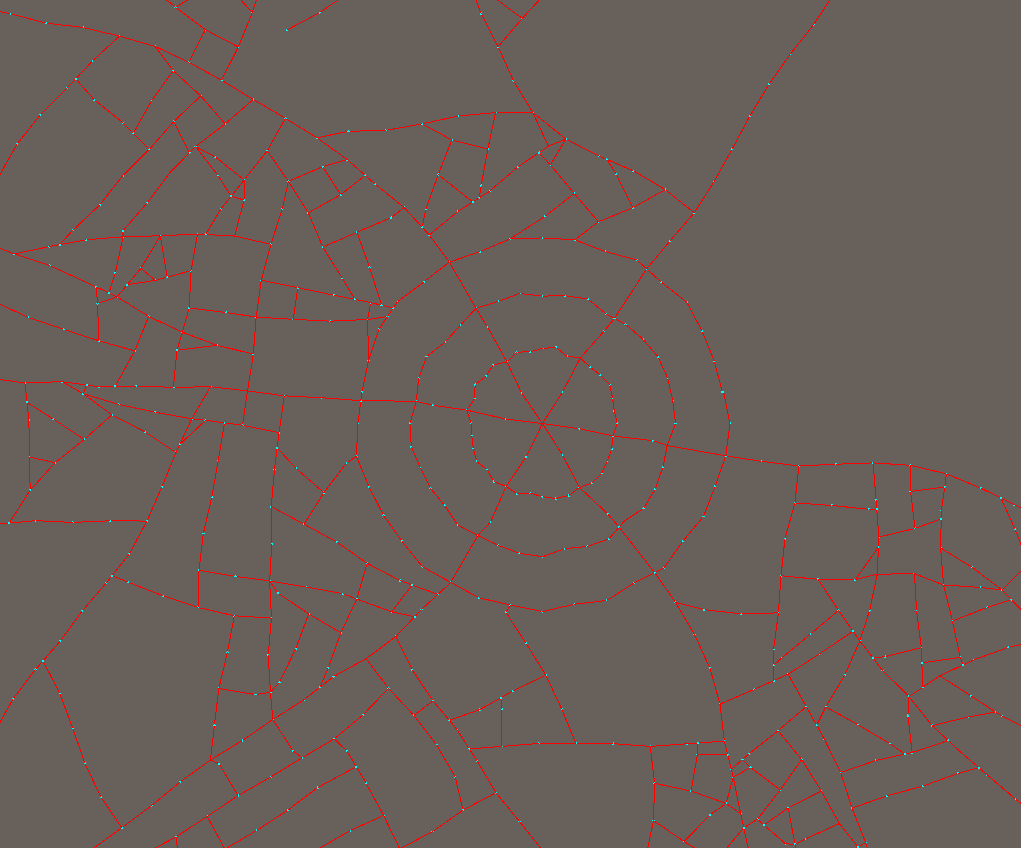
\includegraphics[width=0.36\textwidth]{figure/road_network_paris.png}
  }
  \caption{Example of agent strategy building a Paris-like city shape.}

  \label{fig:road_network_paris}
\end{wrapfigure}

For example, in Figure~\ref{fig:road_network_paris}, the road generator started by creating a ParisAgentFactory, which takes the city position and radius as input, and spawns multiple Agents depending on random variables within the bounds of the input.
The Agents are also given a Paris-like strategy, which instructs the Agents to generate rings around the city center as well as main roads extending outwards.
This particular strategy was configured to have a very aggressive branching, which in turn produces lots of intersections.


%% Intersection logic %%

\begin{wrapfigure}[13]{r}{0.4\textwidth}
  \centering
  \raisebox{0pt}[\dimexpr\height-1\baselineskip\relax]{
    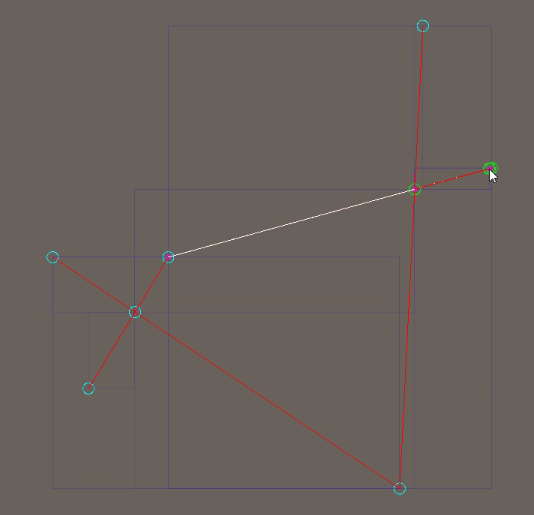
\includegraphics[width=0.36\textwidth]{figure/road_intersection.png}
  }

  \caption{Road intersection and R-Tree bounding boxes}

  \label{fig:road_intersection}
\end{wrapfigure}

While Agent strategies handle how the Agent moves around in the world, it is not what decides how the roads should be placed.
When the Agent decides to place a road, it will attempt to find nearby nodes to snap to by searching in multiple ways.
If no nodes to snap to are found, it will create a road between its last position and its new position, and any roads that exist on the path there in between will be combined into an intersection.
Figure~\ref{fig:road_intersection} demonstrates the intersection created after an Agent attempts to cross another road, as well as an optimization technique making use of an R-Tree. %TODO: REFERENCE

The R-Tree is necessary to quickly search for intersecting roads by avoiding to iterate over all nodes in the road network, or else the performance would result in an unusable application.
Each node is placed in the R-Tree with a bounding box that encapsulates each connecting node.
It is the RoadNetwork that is responsible for handling these cases when nodes are connecting, not the Agents.
When two nodes are connected, the road network will search for nearby nodes that intersect with the bounding box of the new connection, as well as a snap radius which is declared in the Agent configuration.

Furthermore, there are a few cases where it is preferable to not create new nodes for Agents, but rather snap to nearby nodes or network edges.
The algorithm tests for four different cases, visualized in Figure~\ref{fig:road_connection_cases}.

\begin{figure}[H]
  \centering

  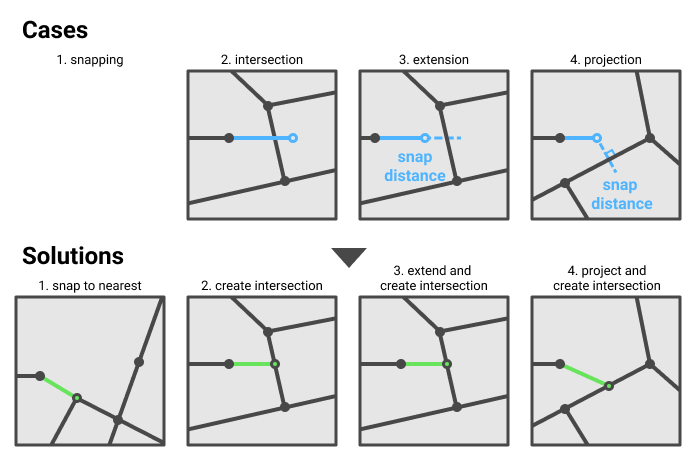
\includegraphics[width=0.8\textwidth]{figure/road_connection_cases.png}
  \caption{Four different cases that are handled in the road network connection logic.}

  \label{fig:road_connection_cases}
\end{figure}

The solutions to the first three cases are similar to those found in CityGen, but it was not enough since it often happened that nodes still appeared close to roads without creating an intersection. % TODO: REFERENCE
To combat this, the solution in the fourth case was added.
\begin{CaseEnum}
  \item The algorithm searches for nodes along the path to the new node, as well as within a radius around the node.
  The distance it searches for is defined in the Agent configuration, which any strategy can define.
  If a node is found, a connection between the previous node and that node will be made, making sure to re-run the algorithm in case paths are blocking.

  \item When there is a road between the origin node and the destination node, a new node will be created, splitting the road where the intersection point is.
  The destination node is then discarded, but note that in Figure~\ref{fig:road_intersection}, the destination node was \textbf{not} discarded.
  In the project, however, the Agent will always stop at the intersection point rather than walk past it.

  \item There are cases where an Agent lands just slightly before another road, but not near enough any other nodes.
  In these cases, the best approach is attempting to extend the node forward a certain distance (the snapping distance), and check if any other roads are intersecting.
  If any are found, split the road at the intersection point and connect the origin node to the intersection node.

  \item The final case occurs when the angle of approach relative to another road is small enough that the extension in the previous case will fail because the intersection point is further away than the snapping distance.
  To solve this, the network checks if there are any roads nearby by creating a perpendicular projection onto onto those roads.
  If the distance to that projection point is within the snapping distance, the same solution is applied as in case 3.
\end{CaseEnum}

First, the algorithm will search for nodes along the path to the new node, as well as a radius around the node.
The second test attempts to \textit{``extend''} the node further forward, and if it intersects with an edge, it will create an intersection there.
The last test does another intersection test, but instead of extending the node forward, it will project the node to nearby edges and create an intersection there if it is within the snap radius.


\begin{wrapfigure}[9]{r}{0.3\textwidth}
  \centering
  \raisebox{0pt}[\dimexpr\height-2\baselineskip\relax]{
    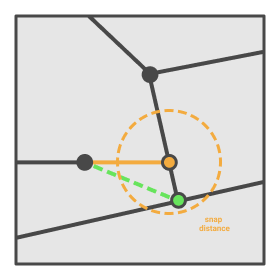
\includegraphics[width=0.26\textwidth]{figure/road_intersection_final_test.png}
  }
  \caption{Example of the test step before intersection node is created.}

  \label{fig:road_intersection_final_test}
\end{wrapfigure}

While these cases solve most of the issues in the road network and make sure Agents are not creating unnecessary roads, it is still not enough to guarantee a good-looking road network.
In cases 2, 3, and 4, one question that came up was \textit{``what happens if the node that was created at the intersection is too close to one of the nodes at the ends of the connection?''}.
The solution to this was that before the node is created and connected, it would take the point of the intersection and check for nearby nodes on the ends of the connection.
If any of those are within the snapping distance, it will snap to the nearest one instead.

%% Highways %%

So far, the generation of main roads within city bounds has been described, but the world also includes highways that connect multiple cities together.
The goal of highway strategies is instructing Agents to generally move towards higher population areas.
When a suitable strategy is implemented that accomplishes this, other strategies can make use of the ability to switch Agent strategies mid-iteration.

The Paris and Manhattan strategies that were used in the project would switch the Agent strategy to a highway one once the Agent stepped outside the boundaries of the city (see Figure~\ref{fig:road_highways}).

\begin{figure}[H]
  \centering

  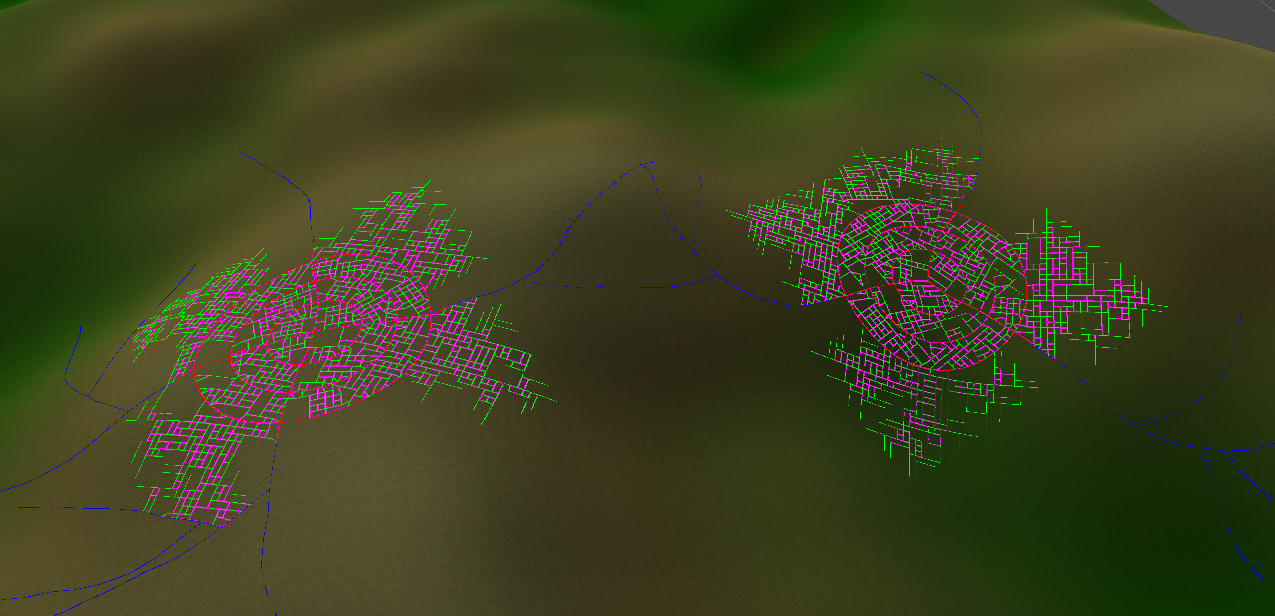
\includegraphics[width=0.8\textwidth]{figure/road_highways.png}
  \caption{Highways created outside the bounds of the city (blue lines), as well as streets (green) with blocks (purple).}

  \label{fig:road_highways}
\end{figure}

The highway strategies that were implemented into the project had a lower probability of branching than other strategies, which produced roads that were longer with fewer exits.
The aim was to produce highways that mimic the structure of highways in the real world, which this logic usually did by connecting cities together with long highways.

\subsection{Street Generation}
The street generator uses the same method as the road generator, which also shows the level of flexibility of the Agent-based approach.
The only difference is that these Agents start on any of the nodes in the road network and uses a street strategy, instead of starting as a city type strategy.

From what the group members have observed, Sweden typically has distinct curved streets in addition to straight intersections, more so than other countries, such as America which generally only have grid-like street blocks.
This indicates that slight variations do exist in the real world, where some streets are curved rather than straight, but in order to limit ourselves in this project, the grid-like streets strategy was chosen as a general strategy for streets of all city types.
However, the base of the road generator and its strategies allows any kind of street pattern to be produced, given a suitable strategy is implemented.
The configuration of the general street strategy can still be configured per city type, which gives a small level of tweaking that matches the given city type better.

Furthermore, the street strategy (and any strategy in general) can watch the population map and react accordingly, either by changing direction or terminating the Agent.
Since the streets is a major part of the overall shape of the city, by watching the population map, the street strategy can directly shape the city according to the population map.
If the population density is too low, it can decide to terminate the Agent, making sure it does not create streets and houses in an area where no population exists.
